\documentclass[a4paper]{article}


\usepackage[utf8]{inputenc}
%\usepackage[T1]{fontenc}
\usepackage[francais]{babel}
\usepackage[left=4.2cm,right=4.2cm,top=3cm,bottom=3cm]{geometry}
\usepackage{graphicx,amsmath,amsthm, amssymb,amsfonts,nicefrac}
\usepackage[svgnames,hyperref]{xcolor}
\usepackage[backref=page, colorlinks, linktocpage, citecolor = blue, linkcolor = blue, urlcolor=blue]{hyperref}
\usepackage{enumitem}
\usepackage{caption}
\usepackage{subcaption}
\usepackage{animate}
\usepackage{zref}

\usepackage{listings}
\usepackage{algorithm}
\usepackage{algorithmic}
\usepackage{color}

\definecolor{dkgreen}{rgb}{0,0.6,0}
\definecolor{gray}{rgb}{0.5,0.5,0.5}
\definecolor{mauve}{rgb}{0.58,0,0.82}

\lstset{frame=tb,
  language=Python,
  aboveskip=3mm,
  belowskip=3mm,
  showstringspaces=false,
  columns=flexible,
  basicstyle={\small\ttfamily},
  numbers=none,
  numberstyle=\tiny\color{gray},
  keywordstyle=\color{blue},
  commentstyle=\color{dkgreen},
  stringstyle=\color{mauve},
  breaklines=true,
  breakatwhitespace=true,
  tabsize=3
}

%%%%%% Notations
\newcommand{\N}{\ensuremath{\mathbb{N}}}
\newcommand{\Z}{\ensuremath{\mathbb{Z}}}
\newcommand{\Q}{\ensuremath{\mathbb{Q}}}
\newcommand{\R}{\ensuremath{\mathbb{R}}}
\newcommand{\tsp}{{}^t\!}

%%%%Theorems, Lemmes etc
\newtheorem{theorem}{Théorème}[subsection]
\newtheorem{corollary}[theorem]{Corollaire}
\newtheorem{lemma}[theorem]{Lemme}
\newtheorem{proposition}[theorem]{Proposition}
\theoremstyle{definition}
\newtheorem{definition}[theorem]{Définition}
\newtheorem{remark}[theorem]{Remarque}
\newtheorem{example}[theorem]{Exemple}
\renewcommand{\proofname}{Démonstration}

%%% lines
\frenchspacing
\linespread{1.1}

\title{\huge Des casinos à l'intelligence articficielle\\[15pt] \small TER M1 DS 2021}
\author{Adrien Maitammar \\ Maxime Le Paumier}
%\email{@}


\begin{document}
\maketitle

\vspace{30pt}

\renewcommand{\contentsname}{Sommaire}
\tableofcontents
 \clearpage
 
 %INTRODUCTION : 
 
\section{Introduction}

\vspace{5pt}

Le premier objectif de ce projet est l'étude de l'algorithme UCB1 (Upper Confidence Bound 1). Cet algorithme a été proposé en 2002 dans le cadre du problème du bandit à $K$ bras.

\subsection{Le problème du bandit à K bras}

Le problème du bandit manchot ou, dans sa version générale, du bandit à $K$ bras, peut se formuler ainsi : un agent est face à des machines à sous (portant le nom de ``bandits manchots'') dont il ne connait pas les récompenses moyennes. Son objectif est alors de maximiser ses gains.

Ce problème est en fait un exemple d'apprentissage par renforcement dans lequel l'agent doit faire des compromis entre l'exploitation (de la machine qui empiriquement lui rapporte le plus) et l'exploration (pour espérer trouver une machine rapportant plus).

L'agent peut bien sûr adopter une approche naïve et jouer la machine maximisant la récompense moyenne sur les coups joués mais  cette stratégie peut le conduire à ignorer certaines machines, qui pourraient être plus intéressantes à jouer. \\
 
Peter Auer, Nicol\`o Cesa-Bianchi et Paul Fischer développent dans leur article \textit{Finite-time Analysis of the Multiarmed Bandit
Problem} une stratégie permettant à l'agent de continuer à explorer les machines tout en maximisant ses gains. Plutôt que de procéder naïvement, celui-ci joue les machines selon la procédure UCB1 ci-dessous.

\vspace{10pt}

\begin{figure}[h]
\noindent\fbox{%
    \parbox{\textwidth}{%
    \textbf{UCB1} \\
     \textbf{Initialisation:} Jouer chaque machine une fois\\
     \textbf{Boucle:} Jouer la machine $j$ qui maximise $\bar{x_j} + \sqrt{ 2\frac{\ln{n}}{n_j} }$ avec $\bar{x_j}$ la récompense moyenne de la machine $j$ jusqu'à présent, $n_j$ le nombre de fois où la machine $j$ a été jouée et $n$ le nombre de coups total.     
    }%
}
\caption{Algorithme UCB1}
\end{figure}

On retrouve dans cette quantité un terme d'exploitation (la moyenne des gains de la machine) ainsi qu'un terme d'exploration donnant plus d'importance aux machines ayant été visitées moins de fois pondéré par $\sqrt{2}$, que l'on appelle constante d'exploration (sur laquelle nous aurons à revenir dans le cadre du jeu de Hex).

\clearpage
\subsection{Le jeu de Hex}

Dans le cadre de ce projet, nous avons cherché à appliquer cet algorithme à un joueur artificiel du jeu de Hex. Il s'agit d'un jeu de société pour deux joueurs dont le but est de relier les deux côtés du plateau correspondant à sa couleur par une ligne continue composée de pièces hexagonales. Avec des règles pourtant simples, la complexité de ce jeu est comparable à celle des échecs, dans le sens où les nombres de coups possibles sont comparables.

\begin{figure}[h]
\centering
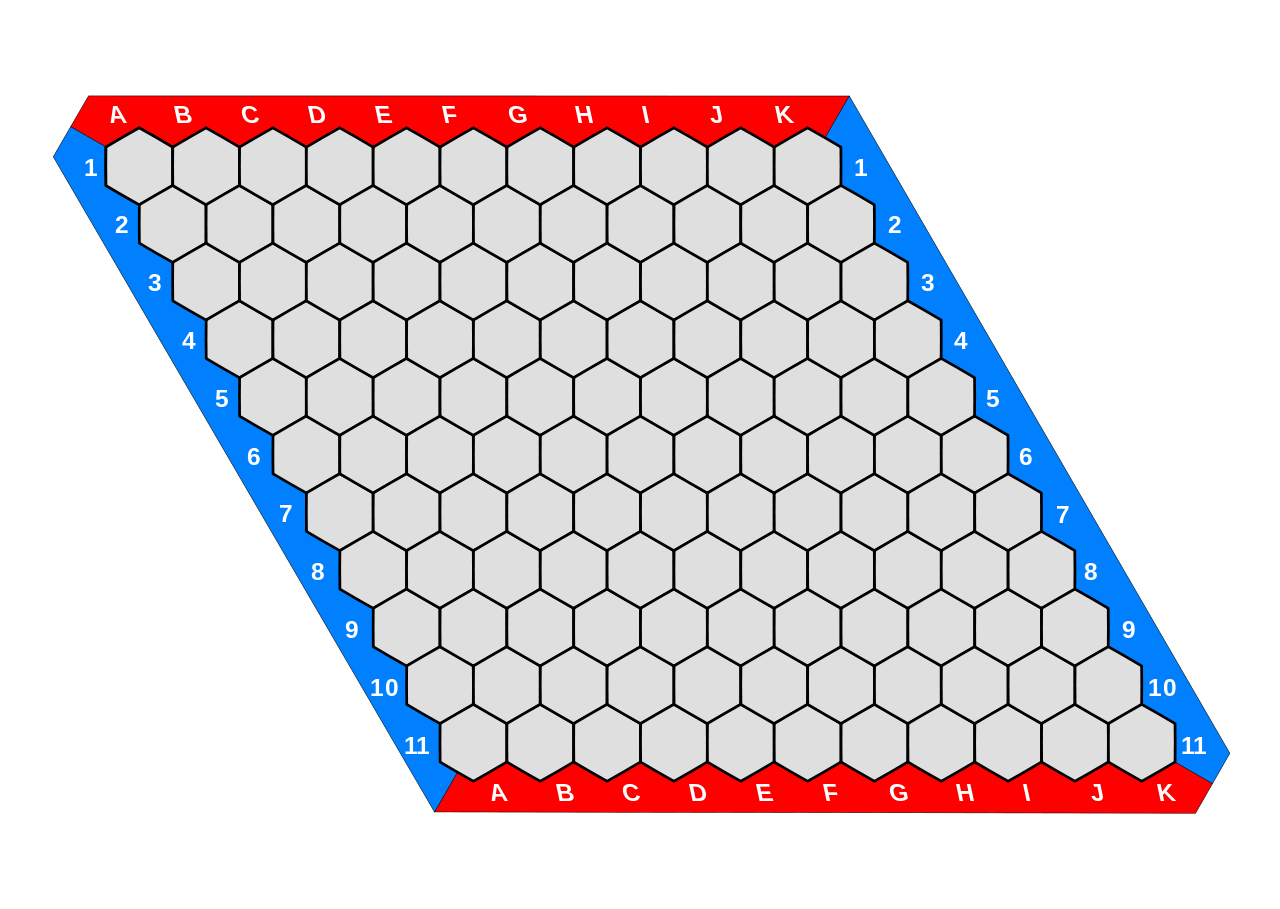
\includegraphics[scale=0.13]{11x11.png}
\caption{Plateau de jeu 11x11}
\end{figure}

Nous verrons dans un premier temps une manière d'implémenter ce jeu sous python puis nous détaillerons deux méthodes de programmation d'un joueur artificiel : une méthode Monte-Carlo puis une méthode UCB appliqué à une recherche arborescente Monte-Carlo que nous appellerons UCT (Upper Confidence bound applied to Trees).

\begin{figure}[h]
\centering
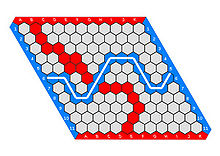
\includegraphics[scale=1]{11x11_gagnant.jpg}
\caption{Configuration gagnante pour le joueur bleu}
\end{figure}




\clearpage
%SECTION 1 : Implémentation du jeu de HEX

\section{Implémentation du jeu de Hex}

\subsection{subsection}


\clearpage
%SECTION 2 : MONTE CARLO

\section{La méthode Monte-Carlo}


\subsection{subsection}


\clearpage
%SECTION 3 : UCB

\section{La méthode UCT}

La méthode Monte-Carlo, bien que relativement efficace, présente pour principal défaut un nombre de calcul très important. Là où cette dernière simule tous les coups possibles, on va plutôt chercher à ne simuler que certains coups, choisis par le critère UCB1, dans le cadre d'une recherche arborescente Monte-Carlo.

\subsection{Recherche arborescente Monte-Carlo}

La recherche arborescente Monte-Carlo ou \textit{Monte Carlo tree search} (MCTS) est un algorithme de prise de décision principalement utilisé dans les jeux \footnote{On peut citer son utilisation dans certains programmes de Go, d'échecs ou de shogi, ou encore le jeu Total War : Rome II}. Le principe de cet algorithme consiste à parcourir l'arbre des possibles dont la racine est l'état actuel du jeu. Chaque noeud est donc une configuration possible et ses enfants représentent les configurations suivantes. Ainsi, on va simuler un certain nombre de coups pour trouver le plus intéressant à jouer.

\subsection{Implémentation de la méthode UCT}

La première étape consiste à sélectionner un noeud à partir d'un noeud parent. Dans la méthode UCT, introduite par Levente Kocsis et Csaba Szepesv\`ari, on utilise le critère UCB1, c'est-à-dire que l'on va choisir le noeud qui maximise $\frac{w}{n} + \sqrt{ 2\frac{\ln{N}}{n} }$ où $w$ est le nombre de parties gagnées après avoir joué ce coup, $n$ le nombre de fois où l'on a joué ce coup et $N$ le nombre de fois où l'on a joué le coup du noeud parent.

\begin{lstlisting}
bestValue = float("-inf")
bestNodes = []

for child in node.children.values():
	nodeValue = child.totalReward / child.numVisits + explorationValue * sqrt(log(node.numVisits) / child.numVisits)
	
       if nodeValue > bestValue:
       	  bestValue = nodeValue
           bestNodes = [child]
        elif nodeValue == bestValue:
           bestNodes.append(child)
             
return random.choice(bestNodes)
\end{lstlisting}

Une fois le noeud sélectionné, et si ce noeud n'est pas un noeud de fin de partie, on procède à une phase d'expansion, lors de laquelle on va choisir aléatoirement un coup à jouer et créer un noeud enfant en conséquence. On va ensuite simuler une partie 	une partie jusqu'à la fin pour obtenir un gagnant. Enfin, on utilise ce résultat lors de la phase de rétropropagation pour mettre à jour les scores des joueurs dans l'arbre. 

\begin{figure}[h]
\centering
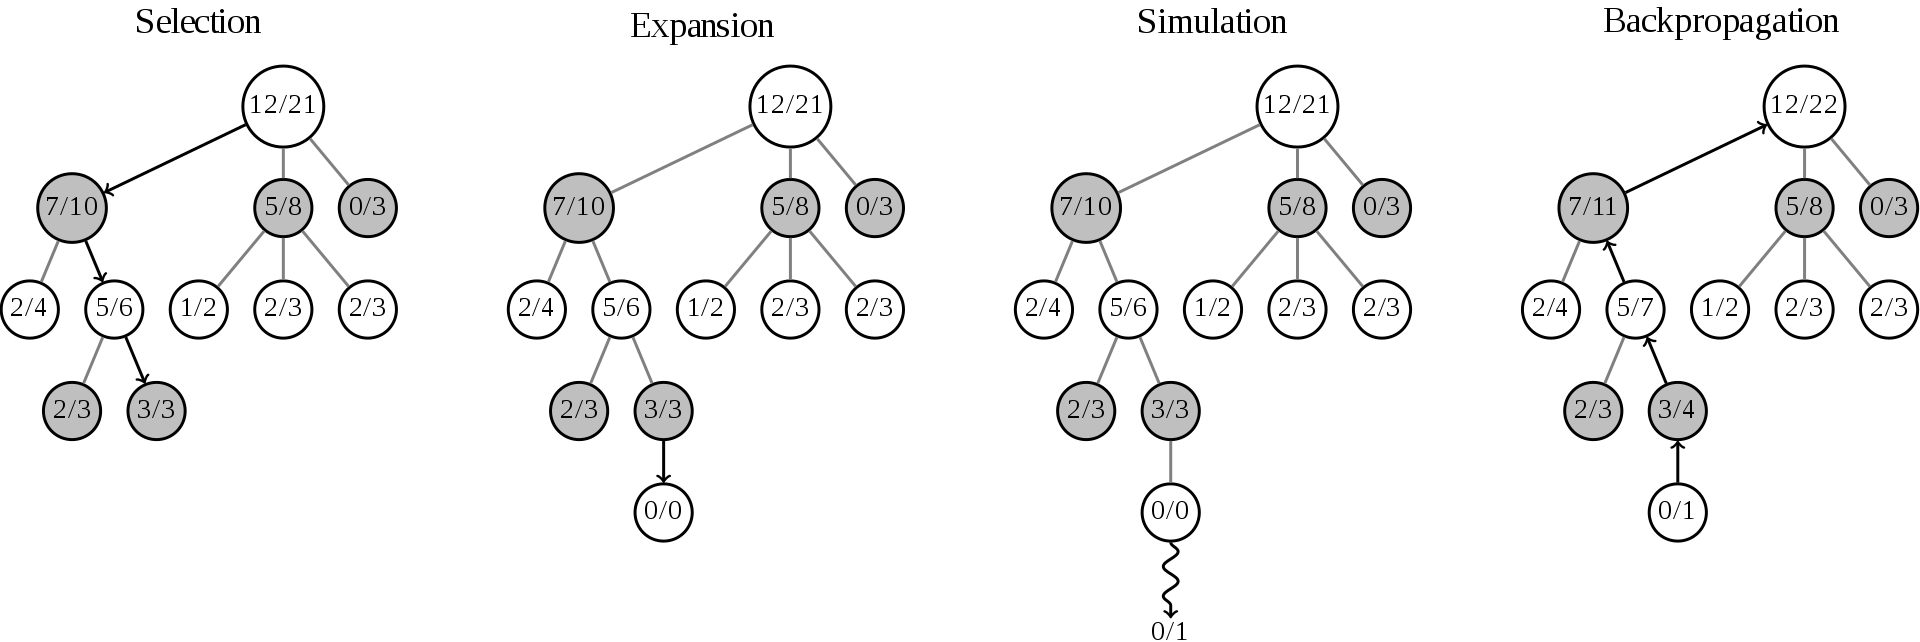
\includegraphics[scale=0.18]{MCTS_wikipedia.png}
\caption{Exemple d'une étape d'un algorithme MCTS. On voit que la partie simulée est perdante pour le joueur qui cherche un coup à jouer. Les noeuds blancs correspondent à un coup joué par le joueur adverse (dont le coup à la racine qui est l'état actuel du plateau). \textit{Source : wikipedia}}
\end{figure}

\subsection{Recherche de la constante d'exploration optimale}



\begin{figure}[h]
\centering
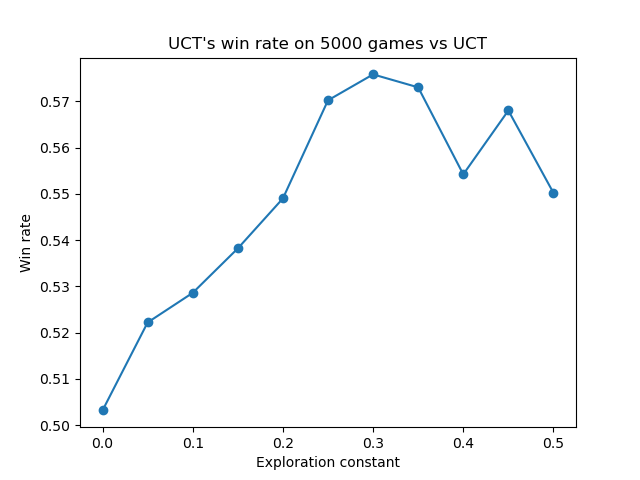
\includegraphics[scale=0.7]{test2.png}
\caption{}
\end{figure}

\subsection{Améliorations possibles}

\clearpage
%\bibliographystyle{myalpha}
\begin{thebibliography}{9}

\bibitem{AZ}
Peter Auer, Nicol\`o Cesa-Bianchi \& Paul Fischer, {\em Finite time Analysis of the Multiarmed Bandit Problem}
\bibitem{AZ}
Levente Kocsis \& Csaba Szepesv\`ari, {\em Bandit Based Monte-Carlo Planning}

\end{thebibliography}

\end{document}